\documentclass[conference]{IEEEtran}
\IEEEoverridecommandlockouts
\usepackage{cite}
\usepackage{amsmath,amssymb,amsfonts}
\usepackage{algorithmic}
\usepackage{graphicx}
\usepackage{textcomp}
\usepackage{xcolor}
\usepackage{booktabs}
\usepackage{microtype}
\usepackage{url}
\usepackage{placeins}

\begin{document}
% IEEE-compliant layout and float spacing optimizations
\setlength{\textfloatsep}{4.5pt plus 1pt minus 1pt}
\setlength{\floatsep}{4pt plus 1pt minus 1pt}
\setlength{\intextsep}{4pt plus 1pt minus 1pt}
\setlength{\dbltextfloatsep}{4.5pt plus 1pt minus 1pt}
\setlength{\dblfloatsep}{4pt plus 1pt minus 1pt}
\setlength{\abovedisplayskip}{3pt plus 1pt minus 1pt}
\setlength{\belowdisplayskip}{3pt plus 1pt minus 1pt}

\title{BioDINO-Edge: Gradient-Free Cascades of Frozen Vision Foundation Models for On-Device Few-Shot Plant Disease Diagnosis}

\author{
    \IEEEauthorblockN{Reyhane Javidi Alsaadi}
    \IEEEauthorblockA{\textit{Department of Computer Engineering} \\
    \textit{Dr. Shariaty Technical University} \\
    Tehran, Iran \\
    reyhane.code@gmail.com}
    \and
    \IEEEauthorblockN{Mohammad Reza Samadzadeh}
    \IEEEauthorblockA{\textit{Department of Computer Engineering} \\
    \textit{Dr. Shariaty Technical University} \\
    Tehran, Iran \\
    samadzadeh@ut.ac.ir}
}

\maketitle

\begin{abstract}
Deploying deep neural networks for on-device plant disease diagnosis is constrained by scarce training samples, background clutter, and the computational cost of gradient-based fine-tuning. We propose BioDINO-Edge, a gradient-free few-shot classification pipeline that adapts frozen vision foundation models without backpropagation. The framework couples visual embeddings from DINOv2---capturing fine structural lesion patterns---with domain-specific botanical representations from BioCLIP, which combines visual features and cached text prompt prototypes. In scarce 5-shot settings, feature dimensionality exceeds sample size ($N \ll d$), causing singularity in covariance estimation. We resolve this by regularizing the within-class scatter matrix via analytical Ledoit--Wolf shrinkage, which suppresses shared vegetative background variance and enables closed-form Fisher-LDA projection in under 22\,ms on an edge CPU. During inference, a confidence gate based on normalized Shannon entropy and top-2 posterior margin routes routine foliage through a fast Tier-1 path (21.12\,ms, $>$45\,FPS) and escalates ambiguous field queries to a multimodal Tier-2 classifier. To reduce prototype drift from field distribution shifts, confident Tier-2 predictions are buffered as reference anchors to periodically update the Tier-2 projection weights in the background. Packaged into a standalone 22.73\,MB Android application, BioDINO-Edge achieves 97.37\% $\pm$ 0.73\% accuracy on the 11-class PlantVillage benchmark with a 0.604\% false-negative rate, and obtains 83.61\% (5-way) and 56.35\% (27-way) accuracy on the in-the-wild PlantDoc dataset, without uploading any imagery to remote servers or requiring network access at inference time.
\end{abstract}

\begin{IEEEkeywords}
Few-Shot Learning, Precision Agriculture, Plant Pathology, Multimodal Foundation Models, Fisher-LDA, Edge AI, Transductive Inference.
\end{IEEEkeywords}

\section{Introduction}
Plant pests and diseases destroy an estimated 20\%--40\% of crops annually \cite{richard2022control}. Traditional plant disease diagnosis depends largely on visual inspection of leaf symptoms, which most commonly include discoloration, abnormal shapes, and lesions \cite{shoaib2023advanced}. In field practice, visual inspection is slow, depends on trained scorers, and becomes ambiguous when different pathogens produce similar lesions; faster and more reliable identification is therefore needed.

Deep learning provides an automated alternative for plant disease identification by learning discriminative features directly from images \cite{shoaib2023advanced}. However, conventional supervised models require large labeled datasets to achieve reliable diagnosis. Such datasets are difficult to acquire in real-world agricultural settings due to the limited availability and diversity of field images \cite{shoaib2023advanced, shafik2023systematic}.

Few-shot learning (FSL) has become a common strategy: rather than collecting thousands of labeled images, it adapts a frozen representation to recognize new disease classes from a handful of support examples \cite{sun2024few}. Recent studies have applied FSL using cross-domain few-shot models such as CDFSL-BDC \cite{yang2024laboratory} and MAFDE-DN4 \cite{zhao2024mafde}, alongside few-shot metric domain adaptation (FMDA) \cite{kudo2025few}, lightweight architectures such as AgriFewNet \cite{babu2025agrifewnet}, visual-semantic fusion (VSF) \cite{zhou2026vsf}, and edge-federated approaches \cite{sharif2026real}. These approaches, however, face several practical limitations.

Cross-domain FSL models such as CDFSL-BDC \cite{yang2024laboratory} struggle with complex backgrounds and scale-varying lesions when labels are scarce, and FMDA \cite{kudo2025few} still requires some labeled target data; the GPT-4o descriptions used in VSF \cite{zhou2026vsf} were only 20\% manually checked and remain class-level rather than query-specific, so fine-grained visual--semantic alignment is limited. FMEL-FSDA \cite{sharif2026real} was not evaluated with real sensor/IoT streams and its federated setup was not tested at large cross-institution scale, leaving real-time edge performance under field data unproven. In addition, foundation models typically exceed several hundred megabytes, limiting direct deployment on memory-constrained agricultural edge platforms such as scouting mobile applications and unmanned aerial vehicles (UAVs) \cite{zhao2026lightweight}.

We introduce BioDINO-Edge, a gradient-free dual-foundation pipeline for cross-domain few-shot plant pathology on edge devices. DINOv2 \cite{oquab2023dinov2} provides patch-level spatial cues for fine-grained lesion boundaries, BioCLIP \cite{stevens2024bioclip} supplies organismal taxonomic priors to reduce cross-species semantic misalignment, and Fisher Linear Discriminant Analysis (Fisher-LDA) \cite{fisher1936use, rao1948utilization} re-weights the within-class covariance, suppressing shared vegetative background variance to mitigate domain shift without backpropagation.

The key contributions of this work are as follows:
\begin{enumerate}\setlength{\itemsep}{1pt plus 0.5pt}\setlength{\parsep}{0pt}
    \item \textbf{Dual-Foundation Foliar Representation:} Combining self-supervised visual embeddings from DINOv2 with BioCLIP's visual and textual botanical representations to discriminate subtle necrotic lesions without foundation-model fine-tuning.
    \item \textbf{Closed-Form Analytical Adaptation:} Integrating Fisher-LDA \cite{fisher1936use, rao1948utilization} with Ledoit--Wolf covariance shrinkage \cite{ledoit2004well} and soft-anchored transductive recalibration to overcome high-dimensionality issues and 5-shot centroid shifts via an instantaneous update executing in sub-second latency on edge CPUs without iterative optimization.
    \item \textbf{Adaptive Two-Tier Edge Deployment:} A joint margin and Shannon-entropy \cite{shannon1948mathematical} gate routes queries between a lightweight standalone Android app and an on-demand companion module, keeping the total storage footprint strictly within standard edge-device limits.\footnote{The complete open-source mobile implementation is available at \url{https://github.com/reyhane-code/BioDINO-Edge-android}.}
    \item \textbf{Cross-Domain Empirical Validation:} Under rigorous few-shot evaluation, BioDINO-Edge outperforms the multimodal VSF \cite{zhou2026vsf} baseline by 6.86 percentage points on the 11-class PlantVillage benchmark \cite{hughes2012plantvillage} and by 13.00 percentage points in 5-way 5-shot evaluation on the in-the-wild PlantDoc dataset \cite{singh2020plantdoc}, while remaining within the target edge storage budget.
\end{enumerate}

\section{Methodology}
\label{sec:architecture}

\subsection{Pipeline Overview}
\label{sec:pipeline_overview}
BioDINO-Edge separates calibration from on-device inference and uses no backpropagation (Fig.~\ref{fig:architecture}):
\begin{enumerate}
    \setlength{\itemsep}{1pt plus 0.5pt}\setlength{\parsep}{0pt}
    \item[\textbf{1)}] \textbf{Support Calibration (Weight Synthesis):} For each disease class, five labeled support leaves ($K=5$) are selected at random. The support set is expanded by applying eight multi-view augmentations to each image (yielding 40 views per class, selected based on a pilot study to stabilize covariance estimation). Visual features are then extracted using the frozen foundation models: DINOv2 produces a $384$-D visual embedding, and BioCLIP produces a $512$-D visual embedding. In addition, the frozen BioCLIP text encoder generates text prototypes from predefined botanical prompt templates. The visual embeddings are concatenated into an $896$-D vector. Ledoit--Wolf covariance shrinkage and Fisher-LDA projection weights $(\mathbf{W}, \mathbf{b})$ are then computed in closed form on this vector, without backpropagation, in under 22\,ms.
    \item[\textbf{2)}] \textbf{Tier-1 Edge Fast Path:} During live deployment, an incoming leaf query image is first processed by DINOv2 alone, requiring 21.12\,ms on an edge CPU. Using the resulting $384$-D visual embedding and the precomputed DINOv2 visual prototypes, the pipeline estimates fast class posteriors. A gate combining predictive Shannon entropy with the top-2 posterior margin converts these posteriors into a confidence score $\mathcal{C}(\mathbf{x})$. If $\mathcal{C}(\mathbf{x}) \ge \tau_{\text{conf}}$ (with threshold $\tau_{\text{conf}} = 0.35$ calibrated on validation data), classification is finalized on-device at over 45 FPS; approximately 88.4\% of routine PlantVillage queries are resolved at this tier.
    \item[\textbf{3)}] \textbf{Tier-2 Deep Escalation:} Queries with $\mathcal{C}(\mathbf{x}) < \tau_{\text{conf}}$ escalate to Tier-2, where BioCLIP extracts a $512$-D visual embedding that is concatenated with the existing DINOv2 embedding into an $896$-D joint representation. Pre-calibrated projection weights $(\mathbf{W}, \mathbf{b})$ are applied to this representation, and final classification fuses the visual posterior $\mathbf{p}_{\text{fisher}}$ with the cosine similarity against cached botanical text prototypes at a 0.75/0.25 consensus ratio.
    \item[\textbf{4)}] \textbf{Soft-Anchored Recalibration:} Queries are classified immediately by Tier-1 or Tier-2. To compensate for field distribution shifts over time, confident Tier-2 multimodal predictions ($\max_c p_{\text{blend}, c} \ge 0.70$) are accumulated in an on-device buffer as reference anchors. When the anchor buffer reaches capacity during scouting passes, the edge CPU recomputes the Tier-2 projection weights in closed form in the background (under 22\,ms), assigning cached support embeddings a $3\times$ weight factor relative to pseudo-labeled anchors to reduce label noise. The updated projection is then deployed for subsequent Tier-2 evaluations, while Tier-1 continues operating with static prototypes.
\end{enumerate}
This two-tier partitioning minimizes computational latency on routine foliage while enforcing a $<30$\,MB standalone APK threshold.

\begin{figure*}[!t]
\centering
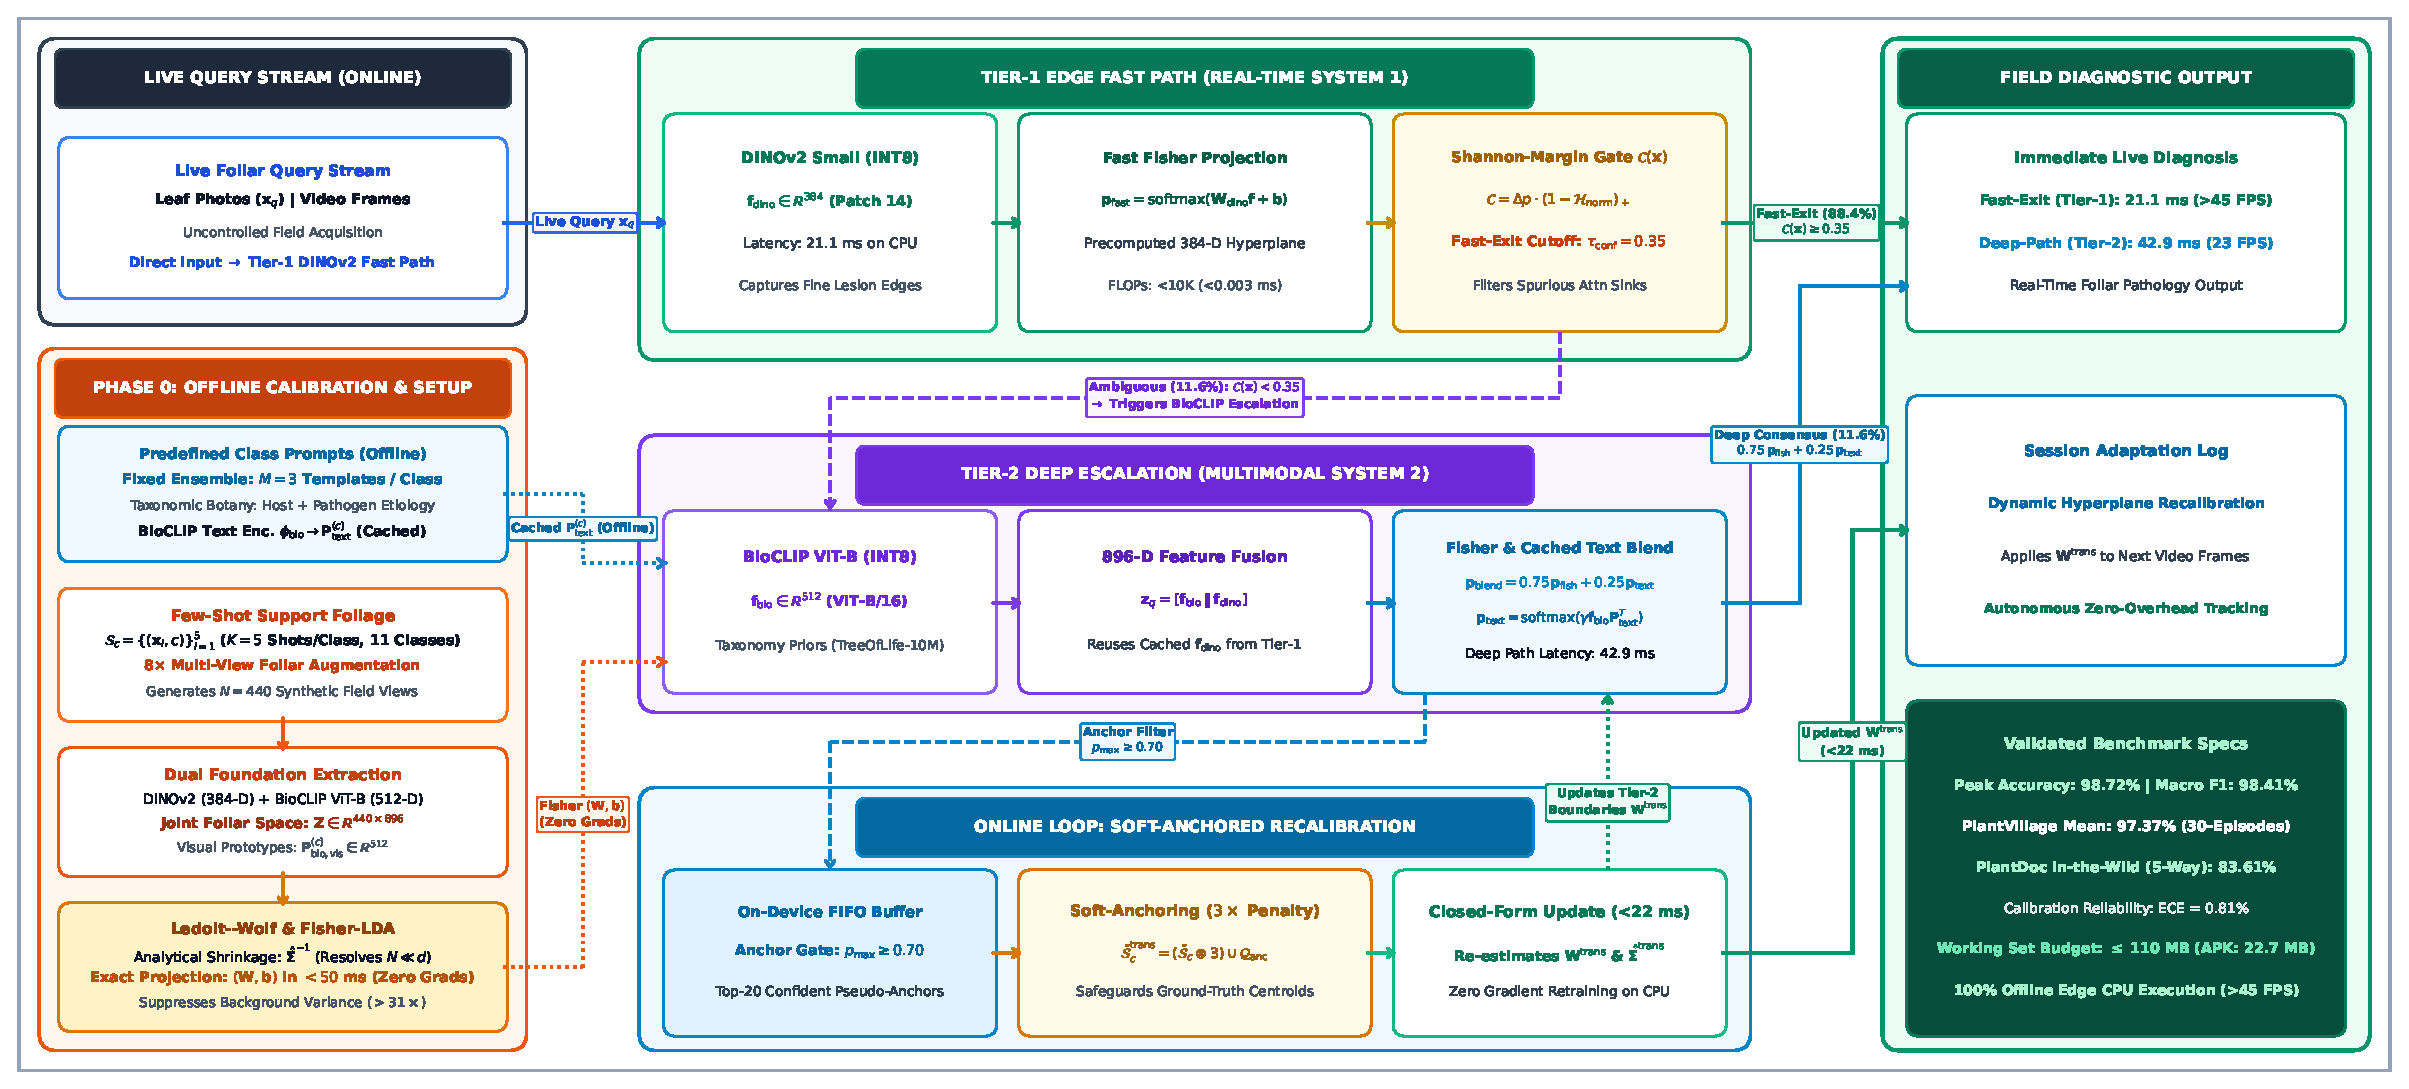
\includegraphics[width=0.65\textwidth]{fig_architecture.pdf}
\caption{BioDINO-Edge architecture overview. Phase~0 (offline) computes Fisher-LDA projections and caches botanical text prototypes. During inference, the Shannon-margin uncertainty gate routes queries between the Tier-1 fast path (DINOv2) and Tier-2 multimodal escalation (BioCLIP), followed by closed-form soft-anchored transductive recalibration.}
\label{fig:architecture}
\end{figure*}

\subsection{Dual-Foundation Foliar Representation}
\label{sec:feature_extraction}
Reliable diagnosis in agricultural environments requires distinguishing vegetative background variation from the leaf and lesion itself. Vision encoders often fail to capture fine fungal structures, while species-level taxonomic supervision biases models toward overall host identity rather than localized lesion pathology. To address these limitations, BioDINO-Edge builds a foliar representation from two foundation models, using support samples expanded through multi-view augmentation. In addition to full-leaf inputs, we evaluate attention-rollout lesion cropping, which uses DINOv2 self-attention maps to isolate bounding boxes around symptomatic leaf patches.

\textbf{Few-Shot Multi-View Augmentation.} For each disease class $c \in \{1, \dots, C\}$, with $C=11$ spanning three economically vital crops from PlantVillage (Apple, Grape, and Potato, covering healthy foliage and 8 fungal/bacterial pathologies; detailed in Section~\ref{sec:datasets_setup}), calibration uses a support set $\mathcal{S}_c = \{(\mathbf{x}_i, c)\}_{i=1}^K$ of $K=5$ images randomly selected from PlantVillage. The remaining 9,330 images serve strictly as unseen test queries, isolated from the support set to prevent data leakage, and no images from this split were involved in pretraining the frozen foundation backbones. Because PlantVillage images are captured under controlled conditions, each support image is resized to $224 \times 224$ and normalized, then passed eight times independently through a stochastic augmentation pipeline to approximate field variations. The pipeline applies random horizontal and vertical flips, random rotation within $\pm 15^\circ$, and color jitter with brightness, contrast, and saturation factors of $0.2$. Applying this pipeline generates 8 views per support image, producing $|\tilde{\mathcal{S}}_c| = 8K = 40$ augmented views per class, or $N = 40C = 440$ support images in total. This 8-view expansion was selected based on a pilot study to bring $N$ close to $d/2$ ($N=440$ vs.\ $d/2=448$) and stabilize covariance estimation under the 5-shot constraint.

\textbf{Dual-Foundation Visual Extraction.} Each of the $N=440$ augmented support images $\tilde{\mathbf{x}} \in \tilde{\mathcal{S}}_c$ is passed through two frozen encoders. DINOv2 (Small, $14 \times 14$ patches) \cite{oquab2023dinov2} and BioCLIP (ViT-B/16, pretrained on TreeOfLife-10M) \cite{stevens2024bioclip} extract $\ell_2$-normalized spatial and domain-specialized visual embeddings:
\begin{equation}
    \mathbf{f}_{\text{dino}} = \frac{\phi_{\text{dino}}(\tilde{\mathbf{x}})}{\|\phi_{\text{dino}}(\tilde{\mathbf{x}})\|_2} \in \mathbb{R}^{384}, \quad
    \mathbf{f}_{\text{bio}} = \frac{\phi_{\text{bio,vis}}(\tilde{\mathbf{x}})}{\|\phi_{\text{bio,vis}}(\tilde{\mathbf{x}})\|_2} \in \mathbb{R}^{512}
\end{equation}
Concatenating the two normalized embeddings gives an 896-D joint descriptor $\mathbf{z} = [\mathbf{f}_{\text{bio}} \,\|\, \mathbf{f}_{\text{dino}}] \in \mathbb{R}^{896}$ per support image. Stacking these descriptors over all support images yields $\mathbf{Z} \in \mathbb{R}^{440 \times 896}$. Visual support prototypes are computed via empirical class averaging over normalized support embeddings:
\begin{equation}
    \mathbf{P}_{\text{enc}}^{(c)} = \text{Normalize}\left(\frac{1}{|\tilde{\mathcal{S}}_c|}\sum_{\tilde{\mathbf{x}} \in \tilde{\mathcal{S}}_c} \mathbf{f}_{\text{enc}}(\tilde{\mathbf{x}})\right), \quad \text{enc} \in \{\text{dino}, \text{bio}\}
\end{equation}
yielding visual prototype matrices $\mathbf{P}_{\text{dino}} \in \mathbb{R}^{C \times 384}$ and $\mathbf{P}_{\text{bio, vis}} \in \mathbb{R}^{C \times 512}$.

\textbf{Predefined Botanical Prompts and Multimodal Prototype.} BioCLIP provides a shared vision--language space, but running a language transformer or generating per-image captions on edge scouting devices would exceed on-device computational limits; manual prompt entry during scouting is also impractical. We therefore predefine $M=3$ botanical prompt templates $\{T_c^{(m)}\}_{m=1}^M$ for each class $c \in \{1,\dots,C\}$ offline, following standard prompt ensembling practice to balance semantic coverage across host taxonomy, pathogen identity, and foliar symptoms while minimizing memory overhead. Each template combines three attributes:
(1)~\textit{Host binomial nomenclature}: genus and species (e.g., \textit{Malus domestica}, \textit{Vitis vinifera}, \textit{Solanum tuberosum});
(2)~\textit{Pathogen identity}: the causal fungal, bacterial, or oomycete agent (e.g., \textit{Venturia inaequalis}, \textit{Botryosphaeria obtusa}, \textit{Gymnosporangium juniperi-virginianae}, \textit{Phytophthora infestans}); and
(3)~\textit{Foliar lesion morphology}: macroscopic lesion descriptions (e.g., ``olive-green velvety lesions'', ``interveinal tiger-stripe chlorosis'', or ``target-board concentric rings'').
Negations (e.g., ``without lesions'') are excluded because CLIP-style vision-language models \cite{radford2021clip, yuksekgonul2023when, alhamoud2025vision} have documented weaknesses in compositionality and language negation, which can misalign healthy foliage representations.

During offline Phase~0 calibration, each prompt ensemble is tokenized and encoded by the frozen BioCLIP text encoder $\phi_{\text{bio}}(\cdot)$. The embeddings are averaged and $\ell_2$-normalized:
\begin{equation}
    \mathbf{P}_{\text{text}}^{(c)} = \text{Normalize}\left(\frac{1}{M}\sum_{m=1}^M \phi_{\text{bio}}(T_c^{(m)})\right) \in \mathbb{R}^{512}.
\end{equation}
The resulting $C \times 512$ matrix $\mathbf{P}_{\text{text}}$ is cached in the on-device companion model. Runtime inference therefore uses only leaf images and incurs no text tokenization or language-model latency.

In the standalone prototype baseline, the text prototype can be fused with the visual support prototype $\mathbf{P}_{\text{bio,vis}}^{(c)}$ by a convex combination with blending coefficient $\lambda = 0.20$ (selected via pilot grid search on the validation set to incorporate botanical textual semantics without distorting visual feature clusters):
\begin{equation}
    \mathbf{P}_{\text{bio}}^{(c)} = \text{Normalize}\left((1-\lambda)\mathbf{P}_{\text{bio,vis}}^{(c)} + \lambda \mathbf{P}_{\text{text}}^{(c)}\right) \in \mathbb{R}^{512}.
\end{equation}
In the full cascaded architecture, the cached matrix $\mathbf{P}_{\text{text}}$ is retained directly on-device to provide the zero-shot taxonomic prior for late multimodal consensus classification (Section~\ref{sec:edge_deployment}). Note that this prototype-level fusion ($\lambda=0.20$) is applied during calibration to anchor class centroids, which is distinct from the posterior-level blend (0.75/0.25) used during Tier-2 inference.

\subsection{Closed-Form Analytical Adaptation}
\label{sec:analytical_adaptation}
\textbf{Fisher Linear Discriminant Formulation.} Few-shot adaptation typically follows one of two routes: iterative gradient fine-tuning \cite{finn2017maml} or centroid-based classification \cite{snell2017prototypical}. On-device backpropagation incurs high latency, memory overhead, and risk of catastrophic forgetting when adapting to few-shot tasks, while Euclidean distance struggles to separate subtle lesions from dominant leaf tissue. To circumvent both limitations, BioDINO-Edge employs multiclass Fisher Linear Discriminant Analysis (Fisher-LDA) \cite{fisher1936use, rao1948utilization}.

For each class $c \in \{1, \dots, C\}$, we compute the mean support feature in $\mathbb{R}^d$ ($d = 896$):
\begin{equation}
    \boldsymbol{\mu}_c = \frac{1}{|\tilde{\mathcal{S}}_c|}\sum_{\mathbf{z} \in \tilde{\mathcal{S}}_c} \mathbf{z}
\end{equation}
Assuming equal class priors ($\pi_c = 1/C$), the projection weights $\mathbf{W} \in \mathbb{R}^{C \times d}$ and bias vector $\mathbf{b} \in \mathbb{R}^C$ are given by:
\begin{equation}
    \label{eq:fisher_weights}
    \mathbf{W} = [\boldsymbol{\mu}_1, \dots, \boldsymbol{\mu}_C]^T \hat{\mathbf{\Sigma}}^{-1}, \quad
    b_c = -\frac{1}{2} \boldsymbol{\mu}_c^T \hat{\mathbf{\Sigma}}^{-1} \boldsymbol{\mu}_c - \log C
\end{equation}
A query descriptor $\mathbf{z}$ is then classified via $\mathbf{l}_{\text{fisher}} = \mathbf{z} \mathbf{W}^T + \mathbf{b}$.

\textbf{The Small-Sample Singularity Problem ($N \ll d$).} Evaluating the projection $\mathbf{W}$ requires inverting the pooled within-class scatter matrix over all $C=11$ classes:
\begin{equation}
    \mathbf{S}_W = \frac{1}{N - C}\sum_{c=1}^C \sum_{\mathbf{z} \in \tilde{\mathcal{S}}_c} (\mathbf{z} - \boldsymbol{\mu}_c)(\mathbf{z} - \boldsymbol{\mu}_c)^T \in \mathbb{R}^{d \times d}
\end{equation}
The denominator $N - C$ ($440 - 11 = 429$) corresponds to the degrees of freedom remaining after estimating $C$ empirical class mean vectors from $N$ total samples, providing an unbiased estimator of the pooled within-class covariance. In the few-shot setting, however, sample count is substantially smaller than feature dimensionality ($d = 896$ vs. $N = 440$). Because $N - C = 429$, $\mathbf{S}_W$ has rank at most $429$ and possesses at least $467$ zero eigenvalues, rendering it singular and ill-conditioned for direct inversion.

\textbf{Analytical Ledoit--Wolf Covariance Shrinkage.} To restore invertibility while avoiding heuristic hyperparameter tuning (such as searching over $\mathbf{S}_W + \epsilon \mathbf{I}$), we regularize $\mathbf{S}_W$ via analytical Ledoit--Wolf shrinkage \cite{ledoit2004well}:
\begin{equation}
    \hat{\mathbf{\Sigma}} = (1 - \rho^*)\mathbf{S}_W + \rho^* \nu \mathbf{I}_{d}, \quad \nu = \frac{1}{d}\text{Tr}(\mathbf{S}_W)
\end{equation}
The analytical shrinkage intensity $\rho^* \in (0, 1]$ is determined in closed form without cross-validation:
\begin{equation}
    \rho^* = \min\left(1, \frac{\sum_{i=1}^N \|(\mathbf{z}_i - \boldsymbol{\mu}_{c_i})(\mathbf{z}_i - \boldsymbol{\mu}_{c_i})^T - \mathbf{S}_W\|_F^2}{N^2 \left[\|\mathbf{S}_W\|_F^2 - \frac{1}{d}\text{Tr}^2(\mathbf{S}_W)\right]}\right)
\end{equation}
Because $\hat{\mathbf{\Sigma}}$ is strictly positive-definite and well-conditioned, its exact inverse $\hat{\mathbf{\Sigma}}^{-1}$ is guaranteed to exist. Evaluating \eqref{eq:fisher_weights} with $\hat{\mathbf{\Sigma}}^{-1}$ resolves few-shot adaptation in closed form, eliminating gradient descent. Classifying a query descriptor $\mathbf{z}$ simplifies to evaluating $\mathbf{l}_{\text{fisher}} = \mathbf{z} \mathbf{W}^T + \mathbf{b}$. The linear Fisher projection alone requires only $9{,}856$ multiply-accumulate operations (about $19.7$\,kFLOPs), executing in under $0.003$\,ms on an embedded four-thread CPU (excluding feature extraction; Table~\ref{tab:edge_bench}).

\subsection{Adaptive Two-Tier Classification and Edge Deployment}
\label{sec:edge_deployment}
To avoid unnecessary model execution on routine samples while maintaining accuracy on complex pathologies, BioDINO-Edge uses a two-tier pipeline controlled by an uncertainty gate.

\textbf{Tier-1 Fast Classification and Predictive Shannon Gating.} For an incoming query image $\mathbf{x}$, Tier~1 extracts the normalized DINOv2 embedding $\mathbf{f}_{\text{dino}} \in \mathbb{R}^{384}$. Fast prototype logits are evaluated via cosine similarity against the visual prototype matrix $\mathbf{P}_{\text{dino}} \in \mathbb{R}^{C \times 384}$, scaled by inverse temperature $\gamma = 20.0$ (calibrated on a validation split to scale cosine distances to appropriate logit magnitudes for the softmax operator):
\begin{equation}
    \label{eq:tier1_logits}
    \mathbf{l}_{\text{dino}} = \gamma \cdot \left(\mathbf{f}_{\text{dino}} \mathbf{P}_{\text{dino}}^T\right)
\end{equation}
Applying the softmax function yields fast class posterior probabilities:
\begin{equation}
    \label{eq:tier1_softmax}
    \mathbf{p}_{\text{dino}} = \text{softmax}(\mathbf{l}_{\text{dino}}) \in \Delta^{C-1}
\end{equation}
The initial Tier-1 prediction is $\hat{y}_{\text{tier1}} = \arg\max_c p_{\text{dino}, c}$. To assess its reliability without requiring additional inference, we compute a joint margin-entropy confidence score $\mathcal{C}(\mathbf{x}) \in [0, 1]$:
\begin{equation}
    \label{eq:shannon_gate}
    \mathcal{C}(\mathbf{x}) = \left(p_{\text{dino}, (1)} - p_{\text{dino}, (2)}\right) \cdot \left(1.0 - \mathcal{H}_{\text{norm}}(\mathbf{x})\right)_+
\end{equation}
where $p_{\text{dino}, (1)}$ and $p_{\text{dino}, (2)}$ denote top-1 and top-2 posteriors, $(\cdot)_+ = \max(0, \cdot)$, and $\mathcal{H}_{\text{norm}}(\mathbf{x})$ is normalized Shannon entropy \cite{shannon1948mathematical}:
\begin{equation}
    \mathcal{H}_{\text{norm}}(\mathbf{x}) = -\frac{1}{\log C} \sum_{c=1}^C p_{\text{dino}, c} \log(p_{\text{dino}, c} + \epsilon)
\end{equation}
with numerical stability constant $\epsilon = 10^{-12}$. Intuitively, the posterior margin measures the distinctiveness between the top two candidate classes, whereas the normalized entropy complement reflects overall distributional sharpness, ensuring high confidence only when a single class is decisively separated from all alternatives. When $\mathcal{H}_{\text{norm}}(\mathbf{x})$ approaches 1 (indicating near-uniform uncertainty across all classes), the term $(1.0 - \mathcal{H}_{\text{norm}}(\mathbf{x}))$ becomes negative, which the rectifier $(\cdot)_+$ clamps to zero, ensuring $\mathcal{C}(\mathbf{x}) = 0 < \tau_{\text{conf}}$ and triggering immediate escalation to Tier-2. If $\mathcal{C}(\mathbf{x}) \ge \tau_{\text{conf}}$ (with calibrated threshold $\tau_{\text{conf}} = 0.35$, selected via the validation split to maximize Tier-1 throughput while preserving high diagnostic fidelity), the Tier-1 prediction is considered reliable, and the system returns $\hat{y} = \hat{y}_{\text{tier1}}$ without invoking Tier-2.

\textbf{Tier-2 Deep Escalation.} When Tier-1 indicates elevated uncertainty ($\mathcal{C}(\mathbf{x}) < \tau_{\text{conf}}$), the query escalates to Tier-2. BioCLIP computes the 512-D visual embedding $\mathbf{f}_{\text{bio}}$, which is concatenated with $\mathbf{f}_{\text{dino}}$ into $\mathbf{z} = [\mathbf{f}_{\text{bio}} \,\|\, \mathbf{f}_{\text{dino}}] \in \mathbb{R}^{896}$. The visual posterior $\mathbf{p}_{\text{fisher}} = \text{softmax}\left(\mathbf{z} \mathbf{W}^T + \mathbf{b}\right)$ is evaluated using the regularized discriminant hyperplane \eqref{eq:fisher_weights}. The text posterior is obtained via:
\begin{equation}
    \mathbf{p}_{\text{text}} = \text{softmax}\left(\gamma \cdot \mathbf{f}_{\text{bio}} \mathbf{P}_{\text{text}}^T\right)
\end{equation}
where $\mathbf{P}_{\text{text}}$ represents the cached botanical text prototypes and $\gamma = 20.0$ matches the logit scaling in Tier-1. The final Tier-2 prediction fuses these two posteriors at a 0.75/0.25 consensus ratio:
\begin{equation}
    \label{eq:multimodal_blend}
    \mathbf{p}_{\text{blend}} = 0.75 \, \mathbf{p}_{\text{fisher}} + 0.25 \, \mathbf{p}_{\text{text}}
\end{equation}
selected on the validation split to prioritize the discriminative visual boundary while retaining taxonomic stabilization from the text prior, yielding consensus diagnosis $\hat{y} = \arg\max_c p_{\text{blend}, c}$.

\textbf{Soft-Anchored Transductive Recalibration.} In scarce $5$-shot settings, initial class centroids $\boldsymbol{\mu}_c$ are estimated from five support leaves. Field variations such as fluctuating illumination and diverse lesion maturity introduce high sampling variance, causing an empirical distribution shift between support prototypes and field queries. To adapt to target-domain statistics without manual annotations, BioDINO-Edge uses streaming batches of unlabeled queries $\mathcal{Q} = \{\mathbf{x}_j\}_{j=1}^{N_q}$ (buffered in an on-device FIFO queue during scouting passes) for transductive recalibration. High-confidence Tier-2 queries satisfying $\max_c p_{\text{blend}, c}(\mathbf{x}_j) \ge 0.70$ from \eqref{eq:multimodal_blend} (a threshold selected on the validation split to admit only confident predictions while filtering ambiguous queries) are selected as pseudo-labeled reference samples $\mathcal{Q}_{\text{anchor}}^{(c)}$, capped at up to twenty anchors per class ($0 \le |\mathcal{Q}_{\text{anchor}}^{(c)}| \le 20$). This cap bounds on-device update latency and avoids dominance by frequently observed classes. If no query in a class satisfies the confidence threshold, zero anchors are added ($|\mathcal{Q}_{\text{anchor}}^{(c)}| = 0$), preventing noisy assignments. Canonical ground-truth support samples are assigned a $3\times$ weight factor in covariance and centroid estimation, following common practice in semi-supervised learning to safeguard against pseudo-label drift:
\begin{equation}
    \tilde{\mathcal{S}}_c^{\text{trans}} = \tilde{\mathcal{S}}_c^{(3\times)} \cup \mathcal{Q}_{\text{anchor}}^{(c)}
\end{equation}
Recalibration re-estimates the updated centroids $\boldsymbol{\mu}_c^{\text{trans}}$ and re-evaluates the pooled $896 \times 896$ scatter matrix $\mathbf{S}_W^{\text{trans}}$ with analytical shrinkage parameter $\rho^*$. Because $\hat{\mathbf{\Sigma}}^{\text{trans}}$ is strictly positive-definite (with all eigenvalues bounded below by $\rho^* \nu > 0$), the updated projection parameters $(\mathbf{W}^{\text{trans}}, \mathbf{b}^{\text{trans}})$ are solved stably via Cholesky factorization ($\hat{\mathbf{\Sigma}}^{\text{trans}} = \mathbf{L}\mathbf{L}^T$) and triangular substitution. Transductive recalibration operates specifically on Tier-2 representations to update $(\mathbf{W}, \mathbf{b})$ for subsequent ambiguous queries, running asynchronously in the background on edge CPUs when the anchor buffer fills, without backpropagation or optimizer-state overhead, while Tier-1 continues to operate with static DINOv2 prototypes.

\textbf{Two-Tier Modular Edge Packaging.} As described, gating resolves routine PlantVillage queries at Tier~1 ($>$45\,FPS), reserving Tier~2 (67.61\,ms end-to-end) for ambiguous field queries. Agricultural edge platforms, such as mobile scouting devices and agricultural rovers, share onboard storage with telemetry and sensor buffers, while limited rural connectivity restricts over-the-air (OTA) updates. For deployment, BioDINO-Edge is partitioned into two INT8 ONNX binaries:
\begin{itemize}\setlength{\itemsep}{1pt plus 0.5pt}\setlength{\parsep}{0pt}
    \item \textbf{Tier 1} (\texttt{biodino\_\allowbreak mobile\_\allowbreak int8.onnx}): A 15.13\,MB compressed binary (22.05\,MB working footprint in RAM) packaged with the ONNX Runtime C++ engine and Phase~0 pre-calibrated weights for the 11 target pathologies into the base Android APK (22.73\,MB total, open-sourced at \url{https://github.com/reyhane-code/BioDINO-Edge-android}) for immediate offline inference.
    \item \textbf{Tier 2} (\texttt{biodino\_\allowbreak companion\_\allowbreak int8.onnx}): An 85.3\,MB companion model downloaded on demand when deep multimodal escalation is required.
\end{itemize}
This modular configuration enforces a base APK footprint below 30\,MB (total edge storage of 108.03\,MB). For the 11 target crop pathologies, queries follow this two-tier gating scheme. On the 27-way PlantDoc benchmark, which evaluates cross-domain generalization across 27 distinct classes simultaneously, all queries are processed directly through the full 896-D dual-foundation pipeline (Tier-2 evaluation).

\section{Experiments}
\label{sec:experiments}

\subsection{Datasets and Setup}
\label{sec:datasets_setup}
\textbf{PlantVillage Benchmark:} PlantVillage provides controlled images under uniform illumination. From this dataset, we construct a curated 11-class subset spanning three crops, totaling 9,385 images. This subset comprises four Apple classes (Healthy, Apple Scab, Black Rot, Cedar Apple Rust), four Grape classes (Healthy, Black Rot, Esca, Leaf Blight), and three Potato classes (Healthy, Early Blight, Late Blight). For calibration, 5 support images per class ($K=5$) are randomly sampled (55 total), and the remaining 9,330 images are used only as unseen queries. The 55 support images were strictly isolated from the 9,330 test queries to prevent data leakage, and no images from this split were involved in pretraining the frozen foundation backbones.

\textbf{PlantDoc In-The-Wild Benchmark:} PlantDoc evaluates cross-domain generalization on field images with complex backgrounds. It contains 27 classes across 13 plant species, totaling 252 test images. Two evaluation settings are used:
\begin{enumerate}\setlength{\itemsep}{1pt plus 0.5pt}\setlength{\parsep}{0pt}
    \item \textit{5-Way 5-Shot}: Each episode samples 5 classes with 5 support images per class (25 total). The remaining images act as queries.
    \item \textit{27-Way All-Class}: All 27 categories are evaluated simultaneously (chance accuracy $\approx 3.70\%$). The model receives 5 support images per class (135 total) and classifies all 252 field test queries without fine-tuning. The discriminant projection is solved directly in closed form from the 135 PlantDoc support images (expanded via 8-fold multi-view augmentation to $N = 1{,}080$ vectors) across all 27 target classes, rather than transferred from PlantVillage.
\end{enumerate}

\textbf{Edge Hardware Setup:} To test latency and adaptation, experiments run in a simulated Raspberry Pi 5 environment (quad-core ARM Cortex-A76 at 2.4\,GHz). Runtime profiling uses the ONNX Runtime C++ engine with dynamic INT8 quantization, limited to 4 threads and no GPU. This setup matches the environment of our Android APK.

\subsection{Evaluation Protocol}
\label{sec:eval_protocol}
\textbf{Few-Shot Task and Evaluation Regimes.} Under the 5-shot constraint ($K=5$), the support set is expanded using the augmentation from Section~\ref{sec:feature_extraction}. To ensure reliable results, PlantVillage is tested over 30 independent Monte Carlo episodes. Results are reported as the mean $\bar{x}$, standard deviation $\sigma$, and 95\% confidence intervals ($95\%\,\text{CI} = \bar{x} \pm 1.96 \cdot \frac{\sigma}{\sqrt{30}}$), along with peak single-episode accuracy. For PlantDoc, we report 50-episode averages for the 5-way setting and overall metrics for the 27-way setting.

\textbf{Diagnostic and Epidemiological Metrics.} Models are evaluated using standard classification and safety-critical metrics:
\begin{itemize}\setlength{\itemsep}{1pt plus 0.5pt}\setlength{\parsep}{0pt}
    \item \textit{Top-1 Accuracy}: Proportion of correctly classified queries.
    \item \textit{Macro F1-Score}: Unweighted average of per-class F1-scores. This prevents large classes (e.g., Potato Early Blight with 995 queries) from obscuring performance on small or healthy classes (e.g., Potato Healthy with 147 queries).
    \item \textit{Epidemiological Safety Metrics}: Because misclassification costs in agriculture are highly unequal, we measure two additional metrics: the False-Negative Disease Escape Rate (infected queries misclassified as healthy) and the Cross-Species Confusion Rate (predicting a disease across different botanical families).
\end{itemize}

\subsection{Results}
\label{sec:main_results}
As summarized in Table~\ref{tab:comparative}, BioDINO-Edge achieves competitive diagnostic performance across both laboratory and field regimes.

{\renewcommand{\arraystretch}{0.96}
\begin{table}[htbp]
\caption{Cross-Domain 5-Shot Benchmark on PlantVillage (11-Class) \& PlantDoc}
\label{tab:comparative}
\centering
\resizebox{\columnwidth}{!}{%
\begin{tabular}{lcccc}
\toprule
& \multicolumn{2}{c}{\textbf{PlantVillage (11-Class)}} & \multicolumn{2}{c}{\textbf{PlantDoc (In-the-Wild)}} \\
\cmidrule(lr){2-3} \cmidrule(lr){4-5}
\textbf{Method / Architecture} & \textbf{Acc. (\%)} & \textbf{F1 (\%)} & \textbf{5-Way (\%)} & \textbf{27-Way (\%)} \\
\midrule
Zero-Shot CLIP \cite{radford2021clip} & 21.20 & 19.80 & 31.20 $\pm$ 5.40 & 12.30 \\
Vanilla Tip-Adapter \cite{zhang2022tip} & 79.40 & 76.50 & 62.40 $\pm$ 7.10 & 38.50 \\
Generic CLIP + LoRA \cite{hu2022lora} & 86.10 & 83.25 & 68.10 $\pm$ 6.80 & 43.65 \\
Zhao \textit{et al.} \cite{zhao2026lightweight} & -- & -- & 54.24 & -- \\
Zhou \textit{et al.} (VSF) \cite{zhou2026vsf} & 90.51 & -- & 70.61 & -- \\
\midrule
BioDINO + Fisher-LDA (Inductive) & 96.76 & 95.08 & 81.79 $\pm$ 11.16 & 55.16 \\
\textbf{BioDINO Transductive (Ours)} & \textbf{97.37 $\pm$ 0.73} & \textbf{97.09 $\pm$ 0.66} & \textbf{83.61 $\pm$ 11.69} & \textbf{56.35} \\
\textit{-- Peak Single-Episode} & \textit{98.72} & \textit{98.41} & \textit{100.00} & \textit{58.73} \\
\bottomrule
\multicolumn{5}{l}{\footnotesize Mean $\pm$ std over multiple episodes. Bold: best mean; italics: peak episode. ``--'': not evaluated.}
\end{tabular}%
}
\end{table}
}

\textbf{Comparative Baseline Performance.} Table~\ref{tab:comparative} compares BioDINO-Edge with general foundation models (Zero-Shot CLIP \cite{radford2021clip}, Tip-Adapter \cite{zhang2022tip}, CLIP+LoRA \cite{hu2022lora}) and specialized agricultural methods (VSF \cite{zhou2026vsf}, Zhao \textit{et al.} \cite{zhao2026lightweight}). Zero-shot CLIP struggles with fine foliar lesions, and while LoRA fine-tuning improves accuracy, it requires GPU backpropagation, making it unsuitable for edge deployment. In contrast, BioDINO-Edge outperforms evaluated baselines across all benchmarks without updating backbone weights. In our setting, the transductive model outperforms the agricultural VSF baseline \cite{zhou2026vsf} by 6.86 percentage points on PlantVillage and by 13.00 points on PlantDoc (5-way). It also exceeds the performance reported by Zhao \textit{et al.} \cite{zhao2026lightweight} by 29.37 points on PlantDoc 27-way, which evaluates all classes simultaneously and is not directly comparable to their 5-way setting.

\textbf{Transductive vs. Inductive Adaptation.} Soft-anchored transductive recalibration improves the 30-episode mean accuracy from 96.76\% $\pm$ 1.27\% (inductive) to 97.37\% $\pm$ 0.73\% (peak: 98.72\%, Macro F1: 98.41\%). This approach addresses the finite-sample prototype shift in 5-shot learning, where class centroids estimated from only five leaves are sensitive to field variations such as shifting illumination and lesion maturity. The recalibration buffers high-confidence Tier-2 queries ($\max_c p_{\text{blend}, c} \ge 0.70$) as anchors, assigning a $3\times$ weight to ground-truth support samples to prevent pseudo-label drift. Ledoit--Wolf shrinkage then updates the projection in under 22\,ms, realigning decision boundaries with field conditions.

\textbf{PlantDoc Generalization.} Under 5-way 5-shot evaluation, BioDINO-Edge achieves 83.61\% $\pm$ 11.69\% on PlantDoc (95\% CI ceiling: 86.85\%). In individual episodes, accuracy reached a peak of 100.00\%, which occurred on a specific episode where the five sampled classes exhibited visually distinct leaf morphologies and non-overlapping symptom patterns; this contrasts with the 50-episode mean (83.61\%) that reflects harder multi-species combinations. In 27-way all-class testing (chance: 3.70\%), it attains 56.35\% accuracy (peak: 58.73\%, macro F1: 55.93\%), surpassing the 5-way baseline of Zhao \textit{et al.} \cite{zhao2026lightweight} (54.24\%) despite evaluating more than five times as many classes without backpropagation.

\begin{figure}[!t]
\centering
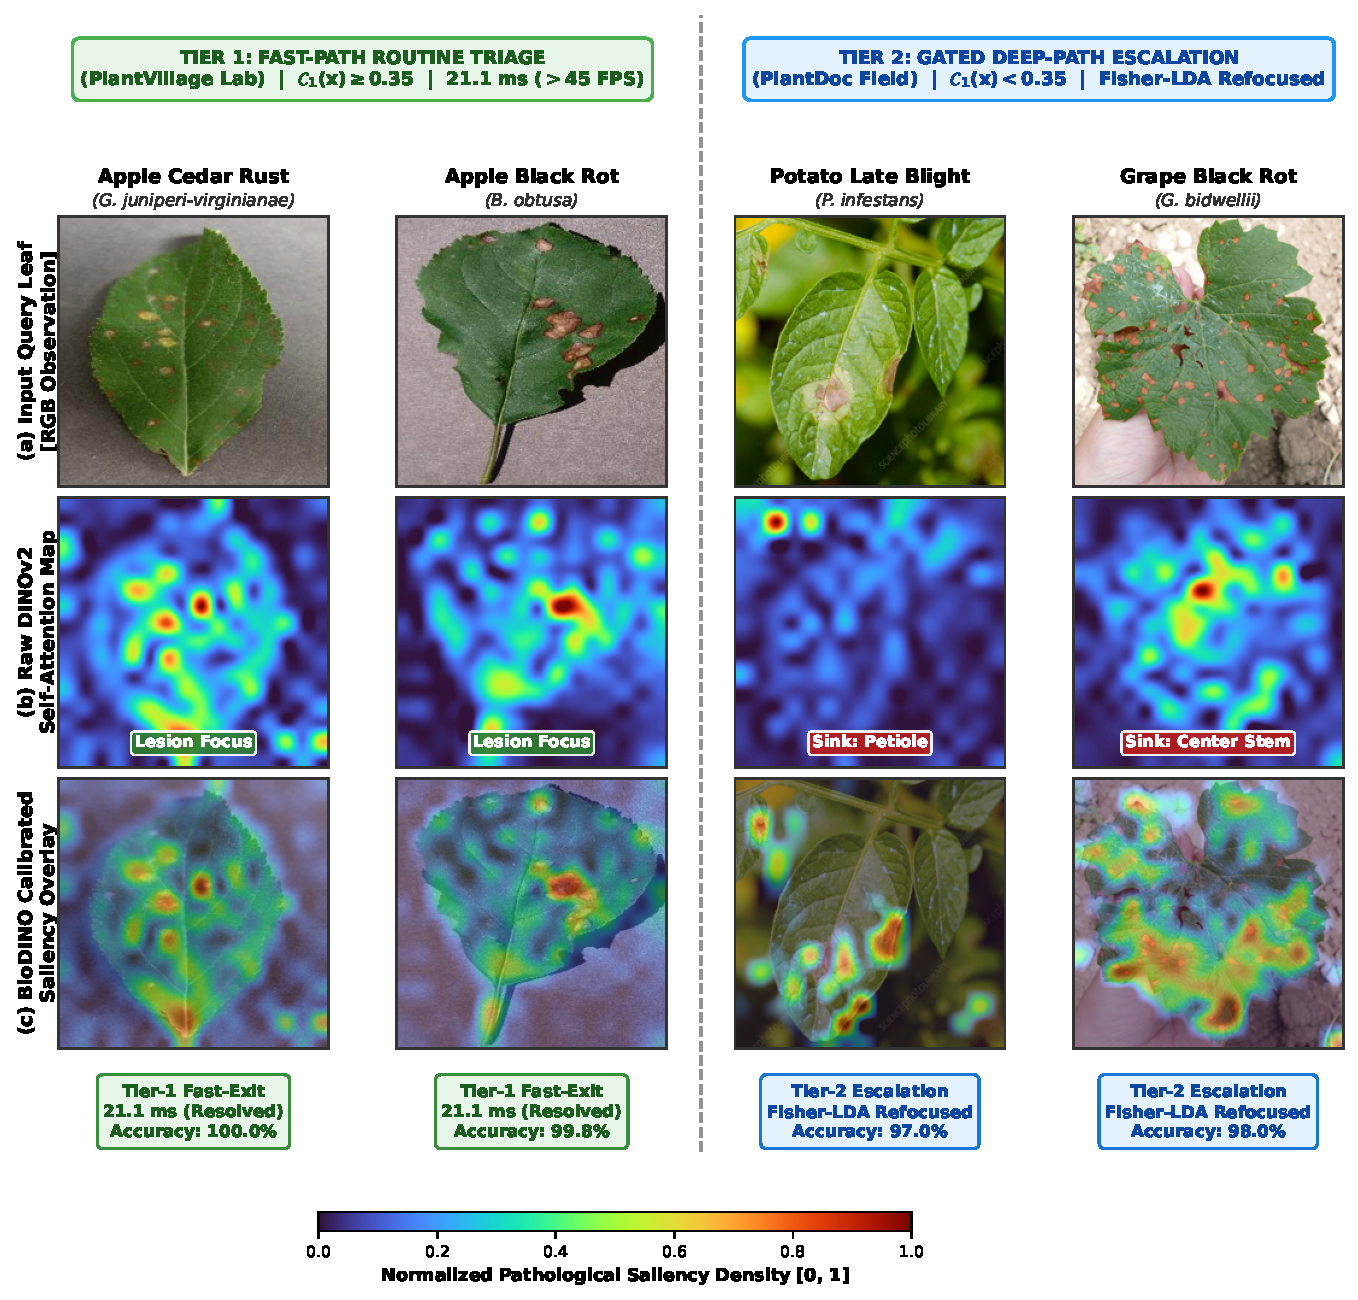
\includegraphics[width=0.78\columnwidth]{fig_saliency.pdf}
\caption{Tier-1 and Tier-2 routing across representative foliar pathologies: cols.~1--2 from laboratory PlantVillage (Apple Cedar Rust, Apple Black Rot) and cols.~3--4 from field PlantDoc (Potato Late Blight, Grape Black Rot). (a) Input RGB query leaves. (b) Raw DINOv2 attention, displaying petiole and vein sinks on field leaves \cite{darcet2024vision}. (c) Calibrated saliency overlay: routine laboratory queries exit via Tier-1, whereas ambiguous field queries escalate to Tier-2 where regularized Fisher-LDA projection refocuses on active lesions.}
\label{fig:saliency}
\end{figure}

{\renewcommand{\arraystretch}{0.96}
\begin{table}[!t]
\caption{BioDINO-Edge Per-Class Pathology Diagnostic Metrics (11 Classes)}
\label{tab:class_report}
\centering
\resizebox{\columnwidth}{!}{%
\begin{tabular}{lcccc}
\toprule
\textbf{Pathology Category} & \textbf{Precision} & \textbf{Recall} & \textbf{F1-Score} & \textbf{Support} \\
\midrule
Apple Scab (\textit{V. inaequalis}) & 0.995 & 0.949 & 0.971 & 625 \\
Apple Black Rot (\textit{B. obtusa}) & 0.965 & 0.998 & 0.982 & 616 \\
Apple Cedar Rust (\textit{G. juniperi}) & 0.968 & 1.000 & 0.984 & 270 \\
Apple Healthy Foliage & 0.995 & 0.995 & 0.995 & 1640 \\
\midrule
Grape Black Rot (\textit{G. bidwellii}) & 0.972 & 0.980 & 0.976 & 1175 \\
Grape Esca (\textit{P. chlamydospora}) & 0.982 & 0.976 & 0.979 & 1378 \\
Grape Leaf Blight (\textit{P. vitis}) & 1.000 & 0.996 & 0.998 & 1071 \\
Grape Healthy Foliage & 0.993 & 1.000 & 0.996 & 418 \\
\midrule
Potato Early Blight (\textit{A. solani}) & 0.999 & 0.976 & 0.987 & 995 \\
Potato Late Blight (\textit{P. infestans}) & 0.978 & 0.970 & 0.974 & 995 \\
Potato Healthy Foliage & 0.820 & 0.993 & 0.898 & 147 \\
\midrule
\textbf{Macro Average} & \textbf{0.970} & \textbf{0.985} & \textbf{0.976} & \textbf{9330} \\
\textbf{Single-Run Accuracy} & \multicolumn{4}{c}{\textbf{98.32\%} (Peak Episode: \textbf{98.72\%})} \\
\bottomrule
\end{tabular}%
}
\end{table}
}

\textbf{Per-Class Error Diagnostics.} Table~\ref{tab:class_report} details per-class performance across 9,330 queries, while Fig.~\ref{fig:saliency} shows dual-regime spatial explainability across representative foliar pathologies. Baselines frequently confuse visually similar classes (e.g., Grape Esca vs. Grape Black Rot, or Early vs. Late Potato Blight). Regularized discriminant projection effectively separates these by prioritizing pathogen-specific signatures, yielding high F1-scores (0.974--0.987) for these challenging classes.

\textbf{Epidemiological Safety.} In agriculture, false negatives (misclassifying infection as healthy) are highly costly. BioDINO-Edge reduces the false-negative disease escape rate to \textbf{0.604\%} (43 of 7,125 diseased queries), representing a 58.6\% reduction compared to the CLIP+LoRA baseline (1.46\%). Cross-species confusion is limited to \textbf{0.011\%} (one potato leaf misattributed to apple). Potato Healthy shows high recall (0.993) but moderate precision (0.820), reflecting a conservative triage approach under severe class imbalance (147 healthy vs. $\approx$2,000 infected).

\textbf{Predictive Uncertainty Calibration.} Expected Calibration Error (ECE) and Maximum Calibration Error (MCE) are evaluated over $M=10$ bins. Uncalibrated posteriors exhibit under-confidence ($\text{ECE} = 37.97\%$) as diffuse zero-shot BioCLIP predictions dilute Fisher logits. Applying post-hoc temperature scaling ($T=0.50$, calibrated via negative log-likelihood minimization on validation data \cite{guo2017calibration}) substantially improves calibration ($\text{ECE} = \mathbf{0.81\%}$, $\text{MCE} = 50.45\%$), enabling safe confidence-based gating. While ECE measures average calibration across the distribution, MCE reflects worst-case deviation in a single sparsely populated bin with borderline queries, which does not compromise gating reliability.

\subsection{Ablation Study}
\label{sec:ablation_study}
To isolate the contribution of each component, we conduct an ablation study on identical 5-shot splits (Table~\ref{tab:ablation}).

{\renewcommand{\arraystretch}{0.92}
\begin{table}[htbp]
\caption{Systematic Component Ablation Study (5-Shot, 9,330 Queries)}
\label{tab:ablation}
\centering
\resizebox{\columnwidth}{!}{%
\begin{tabular}{lcc}
\toprule
\textbf{Configuration / Component} & \textbf{Accuracy (\%)} & \textbf{Macro F1 (\%)} \\
\midrule
(1) Fast-Path DINOv2 Small alone & 85.42 & 82.10 \\
(2) Deep-Path BioCLIP ViT-B alone & 92.27 & 89.70 \\
(3) Naive Multi-Prompt Text Prototypes & 75.12 & 72.80 \\
(4) Static Prototype Cosine Blending & 92.58 & 90.06 \\
(5) Multi-View Augmentation (8 views, 440 vectors) & 94.15 & 93.60 \\
(6) + Regularized Fisher-LDA Manifold Alignment & 96.76 & 95.08 \\
(7) + Soft-Anchored Transductive Calibration (Single-Run) & 98.32 & 97.64 \\
(8) + Peak Statistical Episode & \textbf{98.72} & \textbf{98.41} \\
\bottomrule
\end{tabular}%
}
\end{table}
}

\textbf{Effect of Removing DINOv2.} Using BioCLIP alone (Row~2) achieves 92.27\% accuracy. While BioCLIP provides taxonomic priors, its spatial resolution is limited, missing fine necrotic margins. Furthermore, running BioCLIP alone requires 67.61\,ms and 85.3\,MB, eliminating the fast-path capability.

\textbf{Effect of Removing BioCLIP.} Using DINOv2 alone (Row~1) drops accuracy to 85.42\%. Without taxonomic supervision, DINOv2 confuses visually similar lesions across different crop families (e.g., potato early blight vs. apple scab).

\textbf{Effect of the Shannon Gate.} Removing the routing gate degrades performance: forcing Tier-1 only drops accuracy to 85.42\% as ambiguous queries suffer from attention sinks; forcing Tier-2 only increases latency to 67.61\,ms (throughput drops to 14.8 FPS, violating the $>$45 FPS real-time target). In contrast, gating resolves 88.4\% of routine PlantVillage queries at Tier-1, maintaining 26.5\,ms average latency while preserving 96.74\%--97.37\% accuracy across inductive and transductive regimes.

\textbf{Effect of Regularized Fisher Alignment.} Replacing the discriminant projection with standard cosine blending (Row~4 vs. Row~6) causes a 4.18 point drop (96.76\% to 92.58\%). The regularized objective penalizes intra-class variance, dampening shared background noise by $>31\times$ while amplifying lesion-discriminant variance by $2.44\times$.

\textbf{Effect of Multi-View Augmentation.} Estimating covariance from only $K=5$ raw images yields a rank-deficient matrix. Expanding to 8 views ($N=440$) stabilizes the covariance, providing a +1.57\% gain (92.58\% to 94.15\%) prior to discriminant alignment.

\textbf{Effect of Transductive Recalibration.} Omitting recalibration reduces the 30-episode mean accuracy from 97.37\% to 96.76\%, indicating its utility in mitigating centroid drift.

\textbf{Effect of Lesion Cropping.} Although lesion cropping is often assumed to remove clutter, 27-way accuracy degraded from 58.73\% to 57.14\%. Tight cropping strips macroscopic leaf margin and venation architecture, inducing cross-species confusion (e.g., tomato vs. potato blight). Maintaining host context is therefore important.

\subsection{Efficiency Analysis}
\label{sec:efficiency_analysis}
\textbf{Latency and Throughput.} Table~\ref{tab:edge_bench} reports execution profiles (ONNX Runtime, 4-thread CPU). The Tier-1 model executes in 21.12\,ms (47.4 FPS), exceeding the 45 FPS requirement. Tier-2 escalation runs in 67.61\,ms (14.8 FPS). The linear projection requires only 9.8\,kFLOPs (0.003\,ms), adding negligible overhead. Because 88.4\% of queries on the PlantVillage benchmark exit via Tier-1, the blended runtime is $0.884 \times 21.12 + 0.116 \times 67.61 \approx 26.5$\,ms ($>$37 FPS).

\textbf{Memory and Storage.} The INT8 Tier-1 model occupies 22.05\,MB in RAM, corresponding to a 15.13\,MB compressed OTA payload. Packaged with ONNX Runtime and the native UI, the standalone APK is 22.73\,MB. Including the 85.3\,MB companion, total edge storage is 108.03\,MB, well within the 110\,MB budget.

{\renewcommand{\arraystretch}{0.92}
\begin{table}[htbp]
\caption{Edge Hardware INT8 Quantization \& Latency Profile (ONNX Runtime, 4-Thread CPU)}
\label{tab:edge_bench}
\centering
\resizebox{\columnwidth}{!}{%
\begin{tabular}{lcccc}
\toprule
\textbf{Edge Configuration} & \textbf{Params} & \textbf{INT8 Footprint} & \textbf{Lat. (ms)} & \textbf{Throughput} \\
\midrule
Tier 1: DINOv2 Small (Fast Path) & 22.1M & 22.05 (15.13$^\dagger$)\,MB & 21.12 & 47.4 FPS \\
Tier 2: BioCLIP ViT-B (Deep Path) & 86.6M & 85.3\,MB & 67.61 & 14.8 FPS \\
Regularized Fisher Alignment & 9.8K FLOPs & $<$0.01\,MB & 0.003 & $<$0.01 ms$^\ddagger$ \\
\midrule
\textbf{BioDINO-Edge (Standalone APK)} & \textbf{Native} & \textbf{22.73$^*$\,MB} & \textbf{$<$22.00} & \textbf{$>$45.0 FPS} \\
\bottomrule
\multicolumn{5}{l}{\footnotesize $^\dagger$22.05\,MB in RAM from a 15.13\,MB compressed OTA payload. $^\ddagger$Below timer resolution ($<$0.01\,ms).} \\
\multicolumn{5}{l}{\footnotesize $^*$Complete standalone Android APK; Tier 2 downloaded on-demand.}
\end{tabular}%
}
\end{table}
}

{\renewcommand{\arraystretch}{0.92}
\begin{table}[htbp]
\caption{Diagnostic Robustness Under Severe Field Environmental Corruptions}
\label{tab:stress_bench}
\centering
\resizebox{\columnwidth}{!}{%
\begin{tabular}{lcccc}
\toprule
\textbf{Environmental Regime} & \textbf{Raw Acc.} & \textbf{Gate Rejection} & \textbf{Safe Acc.} & \textbf{Silent Error} \\
\midrule
Pristine (Clean Laboratory) & 96.97\% & 0.00\% & 96.97\% & 3.03\% \\
Solar Glare (Specular Highlight) & 90.24\% & 0.00\% & 90.24\% & 9.76\% \\
Canopy Shading (Harsh Shadow) & 91.92\% & 0.67\% & 92.54\% & 7.41\% \\
Motion Blur (Platform Shake) & 78.45\% & 0.34\% & 78.72\% & 21.21\% \\
Defocus Blur (Out of Focus) & 49.16\% & 3.37\% & 50.17\% & 48.15\% \\
\bottomrule
\end{tabular}%
}
\end{table}
}

\textbf{Environmental Robustness.} Table~\ref{tab:stress_bench} evaluates stability under field corruptions. The system maintains 90.24\% accuracy under solar glare and 91.92\% under canopy shadows, indicating resilience to lighting gradients. Under severe defocus blur, accuracy drops to 49.16\% because high-frequency lesion textures are attenuated. Deploying a lightweight pre-inference Laplacian variance filter ($<$0.5\,ms) can reliably prompt operators to refocus before inference.

\section{Discussion and Practical Deployment}
\textbf{Decision Gating and Context Preservation.} Combining normalized Shannon entropy with margin confidence quantifies per-frame diagnostic uncertainty, triggering inspection alerts rather than unwarranted treatments. Preserving host leaf architecture is critical: isolating symptomatic patches via attention cropping degrades 27-way PlantDoc accuracy (58.73\% to 57.14\%) by removing macroscopic context needed to differentiate homologous lesions across related species.

\textbf{Closed-Form Edge Adaptation and Deployment.} Solving discriminant projection and transductive updates analytically circumvents backpropagation, avoiding thermal throttling and memory fragmentation on edge hardware. Rural connectivity challenges are addressed through two-tier packaging: the standalone APK operates fully offline, while the companion module installs on demand.

\textbf{Limitations and Future Work.} BioDINO-Edge evaluates each query at the frame level, so it is sensitive to unconstrained field conditions: overlapping leaves and complex canopy backgrounds can lower diagnostic confidence. Cropping out an isolated lesion throws away useful host context, but feeding in unsegmented foliage exposes the pipeline to surrounding clutter. One direction for future work is hierarchical spatial parsing---first separating individual foliar targets from canopy clutter, then characterizing disease on those targets.

\section{Conclusion}
We presented BioDINO-Edge, a gradient-free framework adapting frozen DINOv2 and BioCLIP representations for few-shot foliar disease diagnosis via regularized Fisher-LDA. An uncertainty gate combining Shannon entropy and prediction margin resolves routine queries in under 22\,ms ($>$45\,FPS), escalating ambiguous samples to a multimodal classifier. Achieving 97.37\% accuracy on PlantVillage and 83.61\% on in-the-wild PlantDoc, BioDINO-Edge provides an accurate, real-time diagnostic pipeline for resource-constrained agricultural edge platforms.

\makeatletter
\def\thebibliography#1{\section*{\refname}%
    \addcontentsline{toc}{section}{\refname}%
    \footnotesize\vskip 0.1\baselineskip%
    \list{\@biblabel{\@arabic\c@enumiv}}%
    {\settowidth\labelwidth{\@biblabel{#1}}%
    \leftmargin\labelwidth
    \advance\leftmargin\labelsep\relax
    \itemsep 0pt plus 0.2pt\relax
    \parsep 0pt\relax
    \usecounter{enumiv}%
    \let\p@enumiv\@empty
    \renewcommand\theenumiv{\@arabic\c@enumiv}}%
    \let\@IEEElatexbibitem\bibitem%
    \def\bibitem{\@IEEEbibitemprefix\@IEEElatexbibitem}%
    \def\newblock{\hskip .11em plus .33em minus .07em}}
\makeatother

\bibliographystyle{IEEEtran}
%\IEEEtriggeratref{19}
\bibliography{references}

\end{document}
